\chapter{Theoretical Flow Model and Analytical Predictions}
\label{ch:theory}

The full Navier--Stokes equations have no closed-form solution in the widening channel. The geometry is, however, thin and slowly varying, which is exactly the situation that lubrication (Hele-Shaw) theory is designed for \citep{Batchelor1967,Bruus2008}. This chapter derives that theory step by step. It is developed at three levels:
\begin{itemize}
\item T1 is the parallel-plate result used by Delon \emph{et al.} (their Eq.~2);
\item T2 corrects T1 for the drag of the side walls, using the exact solution for a rectangular duct;
\item T3 keeps the two-dimensional character of the planform, which matters near the outlet corner.
\end{itemize}
Each level removes one assumption of the previous one, so comparing them with the CFD shows which physical effect causes which deviation.

\section{Lubrication scaling}
\label{sec:th_scaling}

Let the channel have height $h$, local width $w$ and an axial length scale $\ell=w/|\dd w/\dd x|$ over which the width changes. From \cref{eq:intro_width}, $\ell=L-x$, which is \SI{50}{mm} at the inlet and \SI{15}{mm} at S4. With $\bar U$ the mean velocity, the terms of the $x$-momentum equation scale as
\begin{equation}
\underbrace{\rho u_x\frac{\partial u_x}{\partial x}}_{\rho\bar U^2/\ell}
=-\frac{\partial p}{\partial x}
+\mu\Big(\underbrace{\frac{\partial^2u_x}{\partial x^2}}_{\bar U/\ell^2}
+\underbrace{\frac{\partial^2u_x}{\partial y^2}}_{\bar U/w^2}
+\underbrace{\frac{\partial^2u_x}{\partial z^2}}_{\bar U/h^2}\Big).
\label{eq:th_scaling}
\end{equation}
Relative to the dominant viscous term $\mu\bar U/h^2$, the other terms are of the following order:
\begin{itemize}
\item axial viscous diffusion, $(h/\ell)^2\le10^{-4}$ up to S4;
\item transverse viscous diffusion, $(h/w)^2\le0.02$, except within a distance of order $h$ from a side wall;
\item inertia, $\Rey_h\,h/\ell$. This is smaller than the conservative estimate $\Rey^*=\Rey_h\,h/w$ of \cref{tab:dimensionless} wherever $\ell\ge w$ (i.e.\ for $x\lesssim\SI{43}{mm}$), so it is at most 0.3 and below $3\times10^{-3}$ at the two cell-culture flow rates.
\end{itemize}
Continuity gives $u_z\sim\bar Uh/\ell$. The $z$-momentum equation then shows that $\partial p/\partial z$ is smaller than $\partial p/\partial x$ by a factor $(h/\ell)^2$, so the pressure is uniform across the gap: $p=p(x,y)$. To leading order, the momentum equations reduce to
\begin{equation}
\frac{\partial p}{\partial x}=\mu\frac{\partial^2u_x}{\partial z^2},\qquad
\frac{\partial p}{\partial y}=\mu\frac{\partial^2u_y}{\partial z^2},\qquad
\frac{\partial p}{\partial z}=0 .
\label{eq:th_lub}
\end{equation}
Physically, every vertical column of fluid is in local equilibrium between the pressure gradient and the viscous drag of the floor and the lid. Inertia and the slow change of the planform do not enter.

\section{Local velocity profile}

Because $p$ does not depend on $z$, the first equation of \cref{eq:th_lub} can be integrated twice in $z$:
\begin{align}
\frac{\partial^2u_x}{\partial z^2}&=\frac{1}{\mu}\frac{\partial p}{\partial x}
\;\Rightarrow\;
u_x=\frac{1}{2\mu}\frac{\partial p}{\partial x}z^2+c_1z+c_2 .
\end{align}
No slip on the floor and the lid, $u_x(z=0)=u_x(z=h)=0$, gives $c_2=0$ and $c_1=-\frac{h}{2\mu}\frac{\partial p}{\partial x}$. Hence
\begin{equation}
u_x(x,y,z)=-\frac{1}{2\mu}\frac{\partial p}{\partial x}\,z\,(h-z),
\qquad
u_y(x,y,z)=-\frac{1}{2\mu}\frac{\partial p}{\partial y}\,z\,(h-z).
\label{eq:th_parabola}
\end{equation}
The profile across the gap is a parabola, with its maximum at mid-height,
\begin{equation}
u_{\max}=-\frac{h^2}{8\mu}\frac{\partial p}{\partial x}=\frac32\bar U .
\label{eq:th_umax}
\end{equation}
\Cref{eq:th_umax} links the peak velocity rigidly to the local pressure gradient, and we use it in \cref{sec:val_offset} to test the internal consistency of the CFD.

\section{Depth-averaged flux and the Hele-Shaw equation}

Integrating \cref{eq:th_parabola} across the gap gives the flux per unit width, $\vect q=\int_0^h(u_x,u_y)\,\dd z$:
\begin{equation}
\vect q=-\frac{h^3}{12\mu}\nabla p ,
\qquad \nabla=\left(\frac{\partial}{\partial x},\frac{\partial}{\partial y}\right).
\label{eq:th_darcy}
\end{equation}
This has the form of Darcy's law, with permeability $h^3/12\mu$. Integrating the continuity equation \cref{eq:gov_cont} over the gap, using $u_z=0$ at $z=0$ and $z=h$, gives $\nabla\cdot\vect q=0$. For a constant height this becomes
\begin{equation}
\nabla\cdot\left(\frac{h^3}{12\mu}\nabla p\right)=0
\quad\Longrightarrow\quad
\frac{\partial^2p}{\partial x^2}+\frac{\partial^2p}{\partial y^2}=0 .
\label{eq:th_laplace}
\end{equation}
Within the lubrication approximation the pressure is a harmonic function of the planform coordinates. The side walls carry the condition of zero normal flux, $\partial p/\partial n=0$. This two-dimensional problem is the basis of model T3 (\cref{sec:th_T3}).

\section{One-dimensional solution for the hyperbolic channel (T1)}

If the planform changes slowly, the iso-bars are straight lines across the width, so $p=p(x)$ and $u_y\approx0$. Ignoring the side walls (infinite plates of width $w$), the total flow rate is $Q=w(x)\,q_x$. From \cref{eq:th_darcy},
\begin{equation}
Q=-\frac{w(x)h^3}{12\mu}\frac{\dd p}{\dd x}
\quad\Longrightarrow\quad
\frac{\dd p}{\dd x}=-\frac{12\mu Q}{h^3w(x)} .
\label{eq:th_dpdx_general}
\end{equation}
\paragraph{Pressure gradient.} Substituting the hyperbolic width $w(x)=w_1L/(L-x)$,
\begin{equation}
\frac{\dd p}{\dd x}=-\frac{12\mu Q}{h^3w_1}\left(1-\frac{x}{L}\right).
\label{eq:th_dpdx}
\end{equation}
The pressure gradient therefore falls \emph{linearly} along the axis. The hyperbolic width was chosen precisely so that $1/w(x)$ is linear in $x$.

\paragraph{Pressure distribution.} Integrating \cref{eq:th_dpdx} from 0 to $x$,
\begin{equation}
p(0)-p(x)=\frac{12\mu Q}{h^3w_1}\left(x-\frac{x^2}{2L}\right),
\label{eq:th_p}
\end{equation}
a parabola that is concave downwards and flattens towards the outlet. Over the whole hyperbolic section the pressure drop is
\begin{equation}
\Delta p_{0\to x_t}=\frac{12\mu Q}{h^3w_1}\left(x_t-\frac{x_t^2}{2L}\right)
\equiv R_{\mathrm{hyd}}\,Q,
\qquad R_{\mathrm{hyd}}=\SI{9.16e10}{Pa.s/m^3}.
\label{eq:th_dp}
\end{equation}
With $Q=\SI{0.9998}{\uLmin}$ this gives $\Delta p_{0\to45}=\SI{1.526}{Pa}$ \tagT.

\paragraph{Wall shear stress.} The floor shear follows from \cref{eq:gov_tauw,eq:th_parabola}:
\begin{equation}
\taw=\mu\left.\frac{\partial u_x}{\partial z}\right|_{z=0}=-\frac{h}{2}\frac{\dd p}{\dd x}
=\frac{6\mu Q}{h^2w_1}\left(1-\frac{x}{L}\right)
=\frac{6\mu\bar U}{h}=\frac{4\mu u_{\max}}{h}.
\label{eq:th_tauw}
\end{equation}
This is Eq.~2 of Delon \emph{et al.} (\cref{eq:lit_eq2}). The shear falls linearly from $\tau_1=6\mu Q/(h^2w_1)$ at $x=0$ to $\tau_1/10$ at $x_t$; the ratio is fixed by $w_{\max}/w_1=10$. For \SI{1}{\uLmin}, $\tau_1=\SI{4.47e-3}{Pa}=\SI{0.0447}{\dyncm}$, and for \SI{0.22}{\uLmin}, $\tau_1=\SI{9.84e-4}{Pa}$ \tagT. The identity $\taw=(h/2)|\dd p/\dd x|$ is a momentum balance on a slab of fluid between the floor and the mid-plane. It holds for any locally parabolic flow, whatever the planform, and it is used in \cref{sec:val_cross} to check the CFD.

\paragraph{Shear above the floor.} The viscous shear stress varies linearly across the gap, $\tau(z)=\taw(1-2z/h)$. At $z=\SI{20}{\micro\metre}$, which the reference paper uses as the height of the cell monolayer, $\tau=0.724\,\taw$. The paper's estimate $\tau_{\mathrm{cell}}=3\taw$ \citep{GaverKute1998} instead accounts for the disturbance of the flow by the cell itself, and is not tested here.

\paragraph{Validity of T1.} T1 requires $h/w\ll1$ (no side-wall drag), $\dd w/\dd x\ll1$ (straight iso-bars) and $\Rey^*\ll1$, and it applies only to $0\le x\le x_t$.

\section{Side-wall correction: exact rectangular-duct solution (T2)}
\label{sec:th_sidewall}

T1 treats the channel as infinitely wide, but at the inlet $h/w=0.145$. To quantify the side-wall effect, consider fully developed flow in a rectangle $-w/2\le y\le w/2$, $0\le z\le h$, driven by a constant gradient $G=-\dd p/\dd x$. Keeping the transverse viscous term,
\begin{equation}
\frac{\partial^2u_x}{\partial y^2}+\frac{\partial^2u_x}{\partial z^2}=-\frac{G}{\mu},
\qquad u_x=0\ \text{on all four walls.}
\label{eq:th_poisson}
\end{equation}
\paragraph{Solution.} Write $u_x=u_{pp}(z)+u_h(y,z)$, where $u_{pp}=\frac{G}{2\mu}z(h-z)$ is the parallel-plate solution. The correction $u_h$ satisfies Laplace's equation, vanishes at $z=0$ and $z=h$, and must cancel $u_{pp}$ on the side walls. Expanding $z(h-z)$ in a sine series on $[0,h]$,
\begin{equation}
z(h-z)=\sum_{n\ \mathrm{odd}}\frac{8h^2}{\pi^3n^3}\sin\frac{n\pi z}{h},
\end{equation}
and seeking $u_h=\sum_nB_n\sin(n\pi z/h)\cosh(n\pi y/h)$, which is harmonic and even in $y$, the condition $u_h(\pm w/2,z)=-u_{pp}(z)$ fixes $B_n$. Hence
\begin{equation}
u_x(y,z)=\frac{G}{2\mu}\left[z(h-z)-\sum_{n\ \mathrm{odd}}\frac{8h^2}{\pi^3n^3}\sin\frac{n\pi z}{h}\,\frac{\cosh(n\pi y/h)}{\cosh(n\pi w/2h)}\right].
\label{eq:th_rect_u}
\end{equation}
\paragraph{Flux factor.} Integrating \cref{eq:th_rect_u} over the section gives $Q=\frac{Gwh^3}{12\mu}f(h/w)$, with
\begin{equation}
f\!\left(\frac hw\right)=1-\frac{192}{\pi^5}\frac{h}{w}\sum_{n\ \mathrm{odd}}\frac{1}{n^5}\tanh\frac{n\pi w}{2h}\;\approx\;1-0.630\,\frac hw\quad(w\gg h).
\label{eq:th_flux_factor}
\end{equation}
The side walls reduce the flux at a given gradient. Conversely, at a given flow rate they raise the pressure gradient by $1/f$. With $h/w$ evaluated locally, T2 is
\begin{equation}
\left.\frac{\dd p}{\dd x}\right|_{T2}=\frac{1}{f(h/w(x))}\left.\frac{\dd p}{\dd x}\right|_{T1},
\qquad
\taw^{T2}(y=0)=\frac{\taw^{T1}}{f(h/w(x))}.
\label{eq:th_T2}
\end{equation}
The correction factor $1/f$ is 1.090 at S1, 1.068 at S2, 1.048 at S3, 1.028 at S4 and 1.009 at S5 (\cref{tab:stations}). T2 thus predicts that the CFD shear on the axis should exceed Eq.~2 by about $0.63\,h/w$, most strongly near the inlet.

\paragraph{Transverse distribution of the floor shear.} Differentiating \cref{eq:th_rect_u} at $z=0$,
\begin{equation}
\frac{\tau(y)}{\tau(0)}=\frac{S(y)}{S(0)},\qquad
S(y)=1-\sum_{n\ \mathrm{odd}}\frac{8}{\pi^2n^2}\,\frac{\cosh(n\pi y/h)}{\cosh(n\pi w/2h)} .
\label{eq:th_tau_y}
\end{equation}
Near a side wall, at a distance $\delta=w/2-|y|$ from it, the $n=1$ term dominates. There $\cosh(\pi y/h)/\cosh(\pi w/2h)\approx e^{-\pi\delta/h}$, so that
\begin{equation}
\frac{\tau}{\tau(0)}\approx1-\frac{8}{\pi^2}e^{-\pi\delta/h}.
\end{equation}
The shear is more than a fraction $\varepsilon$ below its core value within the side-wall layer
\begin{equation}
\delta_\varepsilon=\frac{h}{\pi}\ln\frac{8}{\pi^2\varepsilon}
=\SI{0.129}{mm}\ (\varepsilon=\SI{5}{\percent}),\quad
\SI{0.171}{mm}\ (\SI{2}{\percent}),\quad
\SI{0.097}{mm}\ (\SI{10}{\percent}).
\label{eq:th_delta}
\end{equation}
The layer thickness scales with the gap $h$ and is independent of the width. The half-width of the uniform-shear band is therefore $d(\varepsilon)=w/2-\delta_\varepsilon$, and the uniform fraction $2d/w$ must grow as the channel widens. This is the theoretical basis for the imaging zones of Delon \emph{et al.}, and it is tested in \cref{sec:val_transverse}.

\section{Two-dimensional Hele-Shaw model of the full planform (T3)}
\label{sec:th_T3}

T1 and T2 assume straight iso-bars. Near $x=x_t$, however, the wall half-angle jumps from \ang{45} diverging to \ang{45} converging. The flow must turn towards the outlet within a distance comparable to the width (\SI{10}{mm}): the corners become low-velocity regions and the flow along the axis accelerates. To capture this, the depth-averaged equation \cref{eq:th_laplace} was solved on the full planform. The side-wall correction was included in the permeability:
\begin{equation}
\nabla\cdot\left[K(x)\nabla p\right]=0,\qquad K=\frac{h^3f(h/w(x))}{12\mu},
\label{eq:th_T3}
\end{equation}
with these boundary conditions:
\begin{itemize}
\item zero normal flux on the side walls;
\item a uniform inflow giving $Q$ at the inlet of the lead-in;
\item $p=0$ at the outlet.
\end{itemize}
The domain (half planform, symmetry at $y=0$) includes the lead-in, the hyperbola, the \ang{45} walls and the outlet duct. It was discretised with linear finite elements, with \SI{20}{\micro\metre} axial spacing and 81 nodes across the half-width (\cref{app:repro}). The floor shear on the axis is $(h/2)|\nabla p|$ and the mid-plane velocity is $h\tau/(4\mu)$. In the straight lead-in, T3 reproduces the exact rectangular-duct gradient to a relative error of $10^{-5}$. In the slowly varying part of the hyperbola it reduces to T2. It does not resolve the side-wall layer itself, because that is a three-dimensional feature of thickness $\sim h$. \Cref{fig:T3} shows the T3 shear field and its prediction that the axial shear departs from Eq.~2 from $x\approx\SI{40}{mm}$ onwards. The minimum is at $x=\SI{44.1}{mm}$, and at S5 the shear is \SI{54}{\percent} above Eq.~2 \tagT.

\begin{figure}[htbp]
\centering
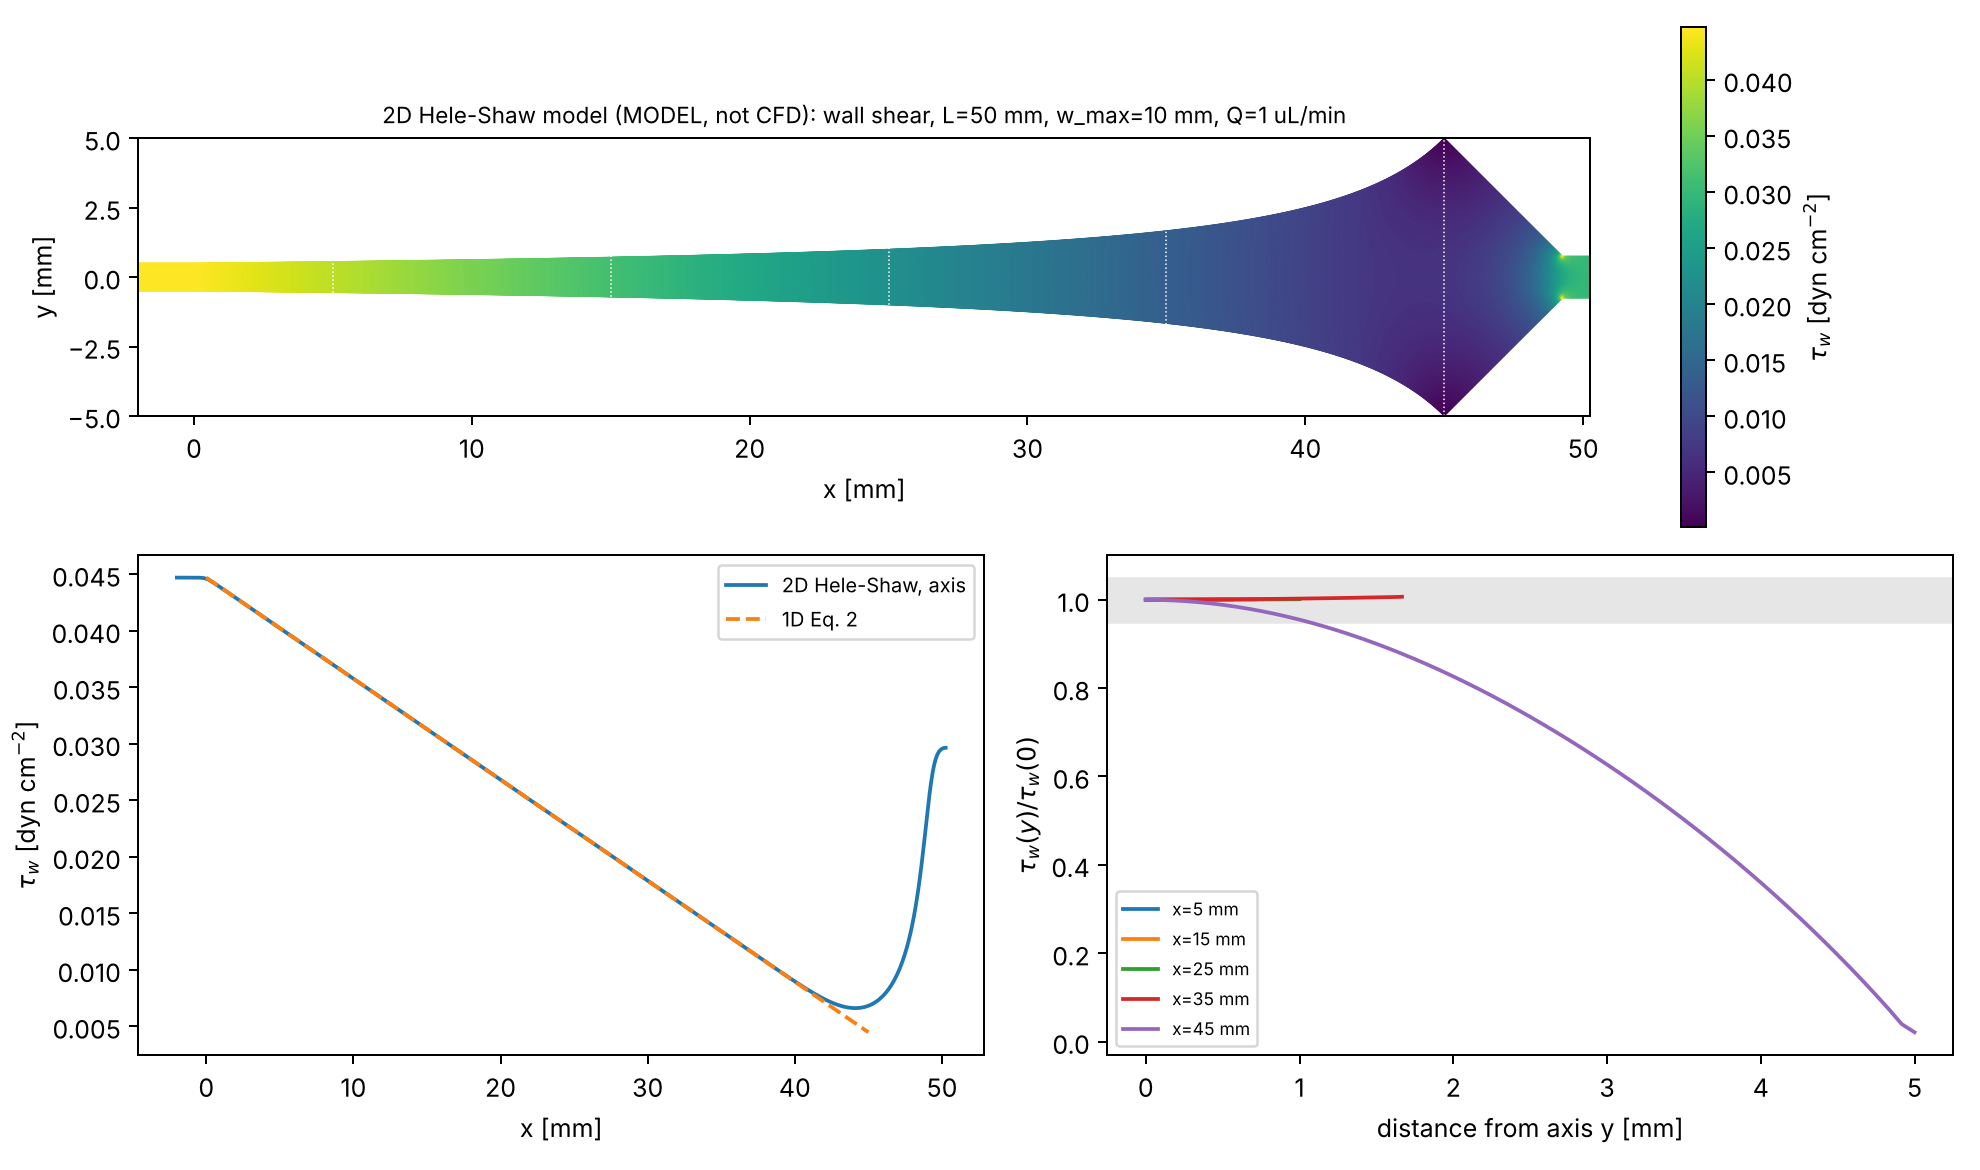
\includegraphics[width=0.95\linewidth]{T3_hs2d_W10_Q1.png}
\caption{Model T3, the two-dimensional Hele-Shaw solution at \SI{1}{\uLmin} \tagT. Top: wall shear on the floor over the planform (\si{\dyncm}). Bottom left: axial shear compared with Eq.~2; the two coincide until $x\approx\SI{40}{mm}$, after which the converging outlet raises the shear. Bottom right: transverse shear profiles normalised by the axis value. They are flat at S1--S4 (T3 has no side-wall layer) and dome-shaped at S5.}
\label{fig:T3}
\end{figure}

\section{Summary of analytical predictions}

\Cref{tab:theory_stations} collects the predictions at the five stations for \SI{1}{\uLmin} ($Q=\SI{0.9998}{\uLmin}$). All quantities are proportional to $Q$. These are the quantities compared with the CFD in \cref{ch:validation}:
\begin{itemize}
\item the axial pressure $p(x)$, the pressure drop and the gradient $\dd p/\dd x$;
\item the centre-line wall shear $\taw(x)$ and its ratio to Eq.~2;
\item the transverse shear profile $\tau(y)/\tau(0)$ and the uniform half-width $d(\varepsilon)$;
\item the mid-plane velocity and the momentum balance $\taw=(h/2)|\dd p/\dd x|$.
\end{itemize}
The parabolic profile $u_x(z)$ of \cref{eq:th_parabola} could not be compared, because the velocity exports contain no $z$ coordinate (\cref{sec:num_exports}).

\begin{table}[htbp]
\centering
\caption{Analytical predictions at the stations, $Q=\SI{0.9998}{\uLmin}$ \tagT. Shear in mPa (\SI{1}{mPa}=\SI{0.01}{\dyncm}). The mid-plane velocity and $d$ at S1--S4 are from T2; at S5 they are from T3.}
\label{tab:theory_stations}
\small
\begin{tabular}{@{}lccccccc@{}}
\toprule
Station & $\taw^{T1}$ & $\taw^{T2}$ & $\taw^{T3}$ & $-\dd p/\dd x|_{T1}$ & $-\dd p/\dd x|_{T2}$ & $u_{\mathrm{mid}}(0)$ & $d$ (\SI{\pm5}{\percent})\\
 & [mPa] & [mPa] & [mPa] & [Pa/m] & [Pa/m] & [mm/s] & [mm]\\
\midrule
S1 & 4.023 & 4.383 & 4.383 & 55.49 & 60.46 & 0.1690 & 0.427\\
S2 & 3.129 & 3.343 & 3.342 & 43.16 & 46.11 & 0.1289 & 0.586\\
S3 & 2.235 & 2.342 & 2.342 & 30.83 & 32.30 & 0.0903 & 0.871\\
S4 & 1.341 & 1.379 & 1.379 & 18.50 & 19.02 & 0.0532 & 1.538\\
S5 & 0.447 & 0.451 & 0.688 & 6.17 & 6.22 & 0.0265 & 1.050\\
\bottomrule
\end{tabular}
\end{table}
